\section{Evaluation}

The contenders:
\begin{enumerate}
\item Run every job on un-tuned on-demand instance (cost and running time)
\item Run every job on nanohub/big-red-2 (running and waiting time)
\item Run on transient, restart every time (cost)
\item SciSpot with early stopping and job sacrificing 
\end{enumerate}

Performance of 3 benchmarks on different types of instance types and bigred2.



\subsection{Preemption likelihood curves}


\subsection{Searching for the best cloud configuration}

\begin{figure}[h]
  \centering
  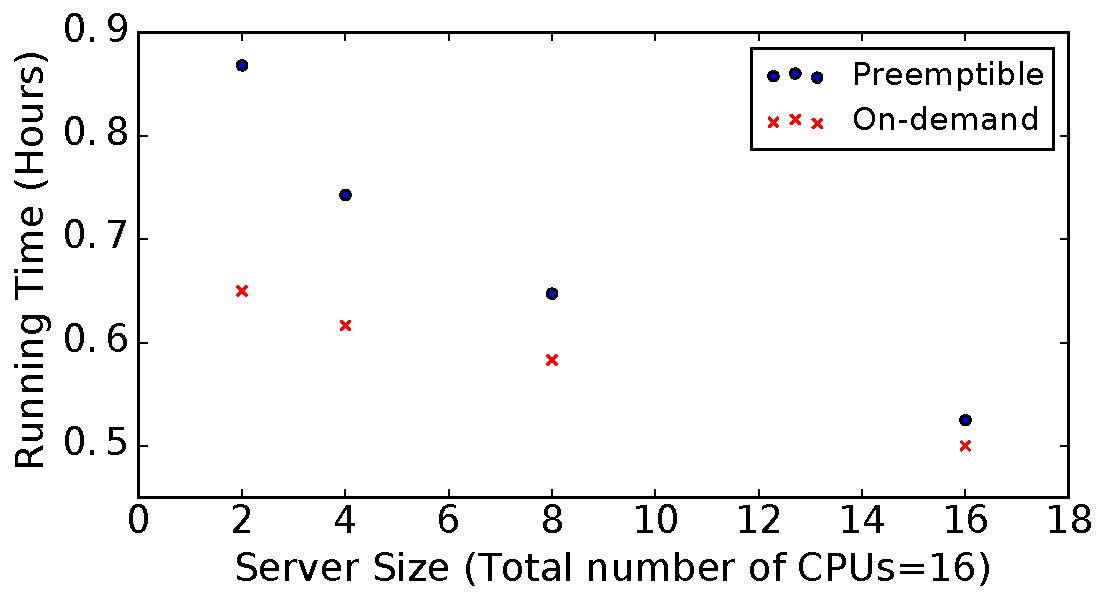
\includegraphics[width=0.4\textwidth]{../graphs/confin_16_time.pdf}
  \caption{confinement running times}
  \label{fig:confin-16-times}
\end{figure}


\begin{figure}[h]
  \centering
  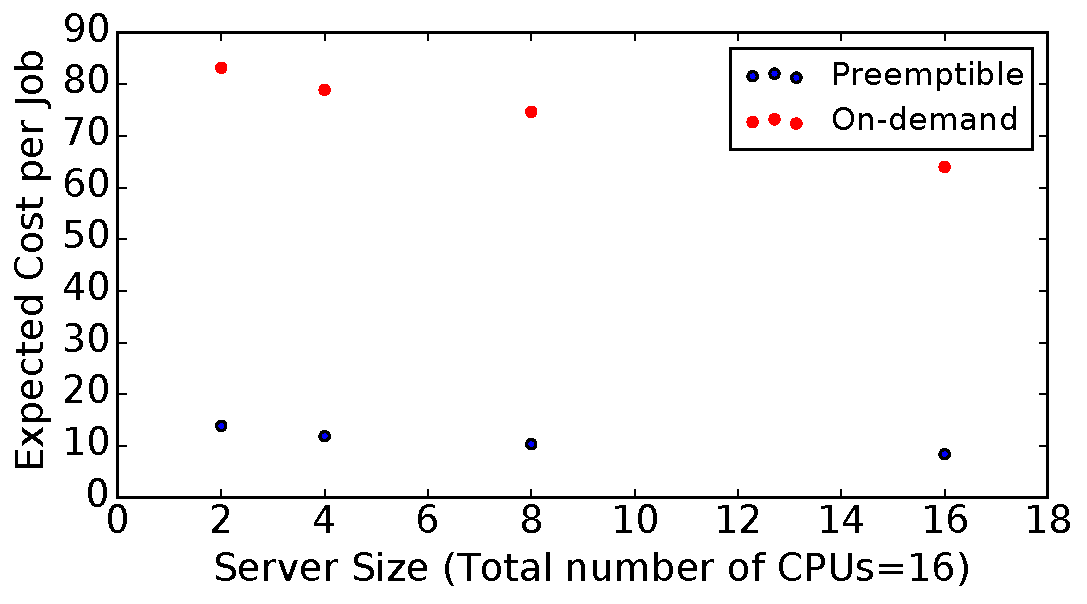
\includegraphics[width=0.4\textwidth]{../graphs/confin_16_cost.pdf}
  \caption{confinement cost}
  \label{fig:confin-16-cost}
\end{figure}

\begin{figure}[h]
  \centering
  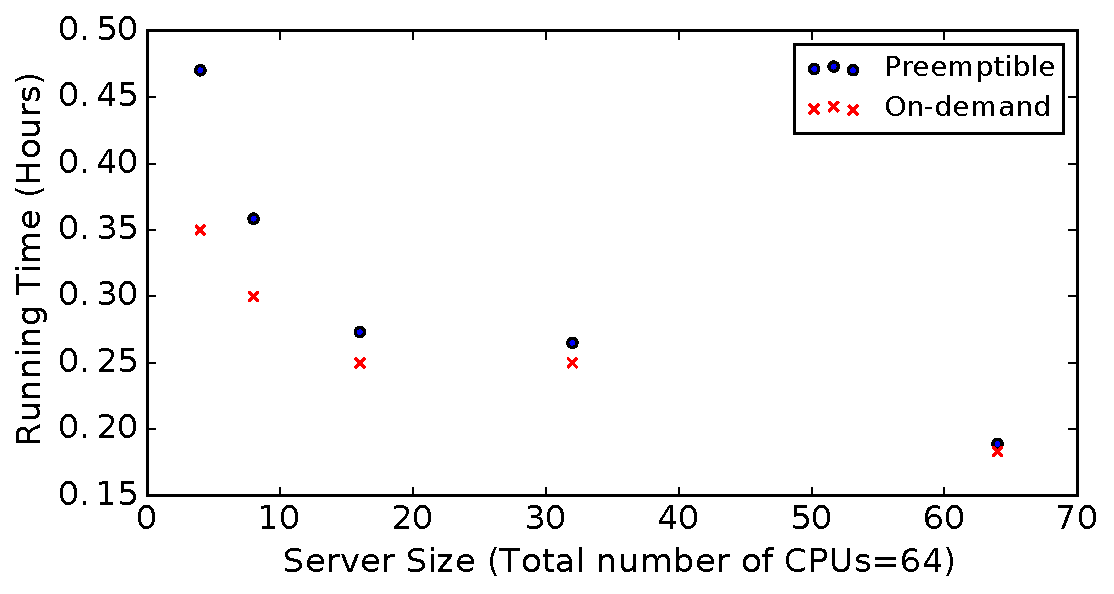
\includegraphics[width=0.4\textwidth]{../graphs/confin_64_time.pdf}
  \caption{confinement running times}
  \label{fig:confin-64-times}
\end{figure}


\begin{figure}[h]
  \centering
  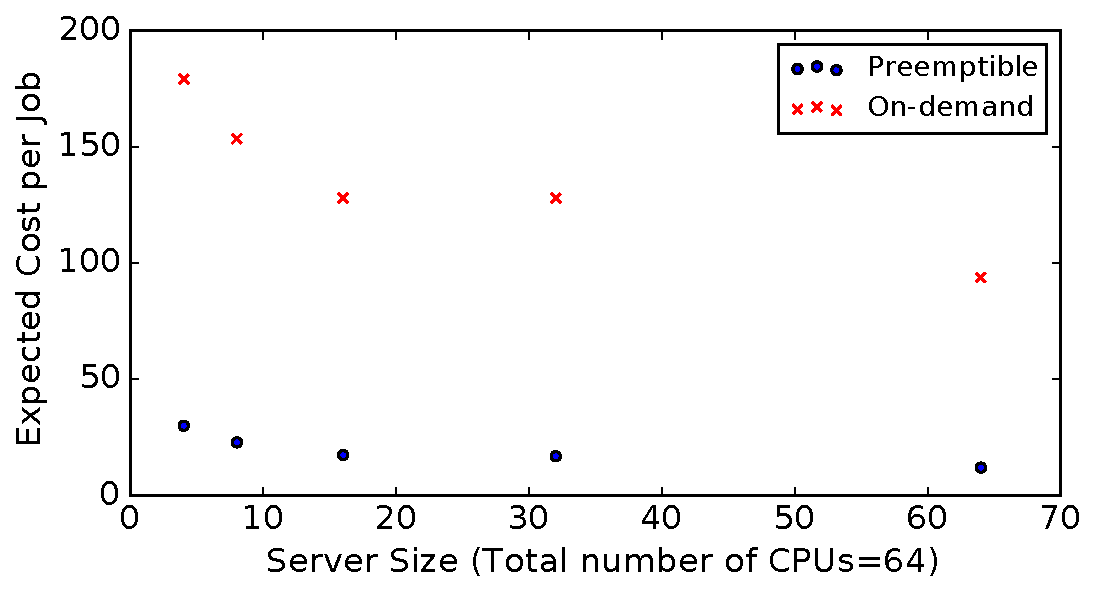
\includegraphics[width=0.4\textwidth]{../graphs/confin_64_cost.pdf}
  \caption{confinement cost}
  \label{fig:confin-64-cost}
\end{figure}



\subsection{Total cost vs. running time graphs}

\subsection{HPC}

\begin{figure}
  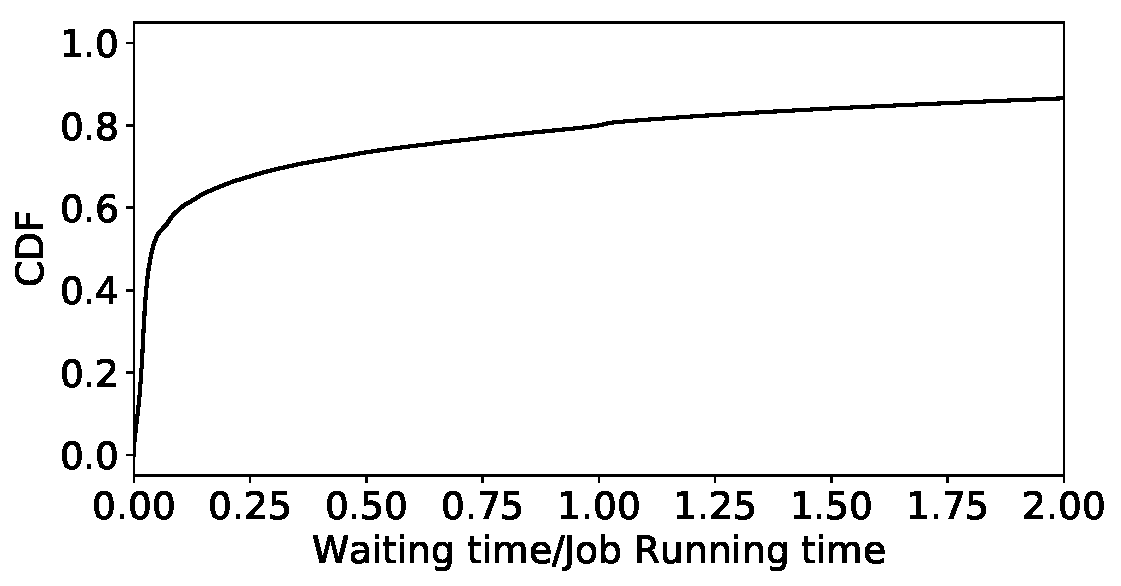
\includegraphics[width=0.4\textwidth]{../data/waiting_all.pdf}
  \caption{Ratio of waiting time to job running time on an HPC cluster. Average is 0.2}
  \label{fig:hpc-wait-cdf}
\end{figure}

% \begin{figure}
%   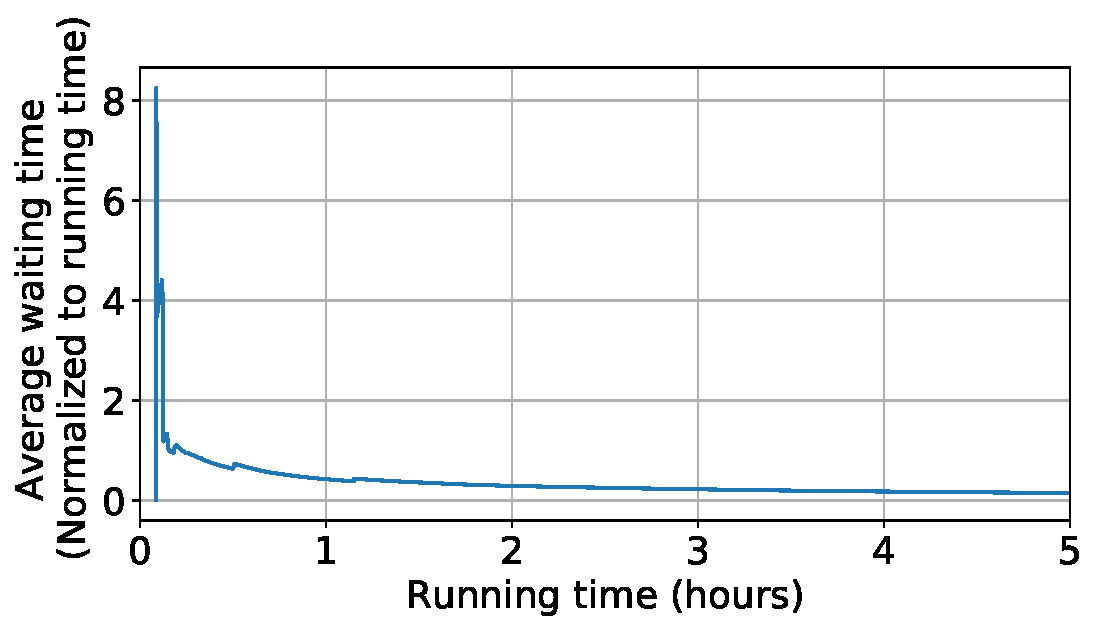
\includegraphics[width=0.4\textwidth]{../data/waiting_cumul.pdf}
%   \caption{The average waiting time (normalized to running time) of jobs of different length.}
%   \label{fig:hpc-wait-cdf}
% \end{figure}


\begin{figure}
  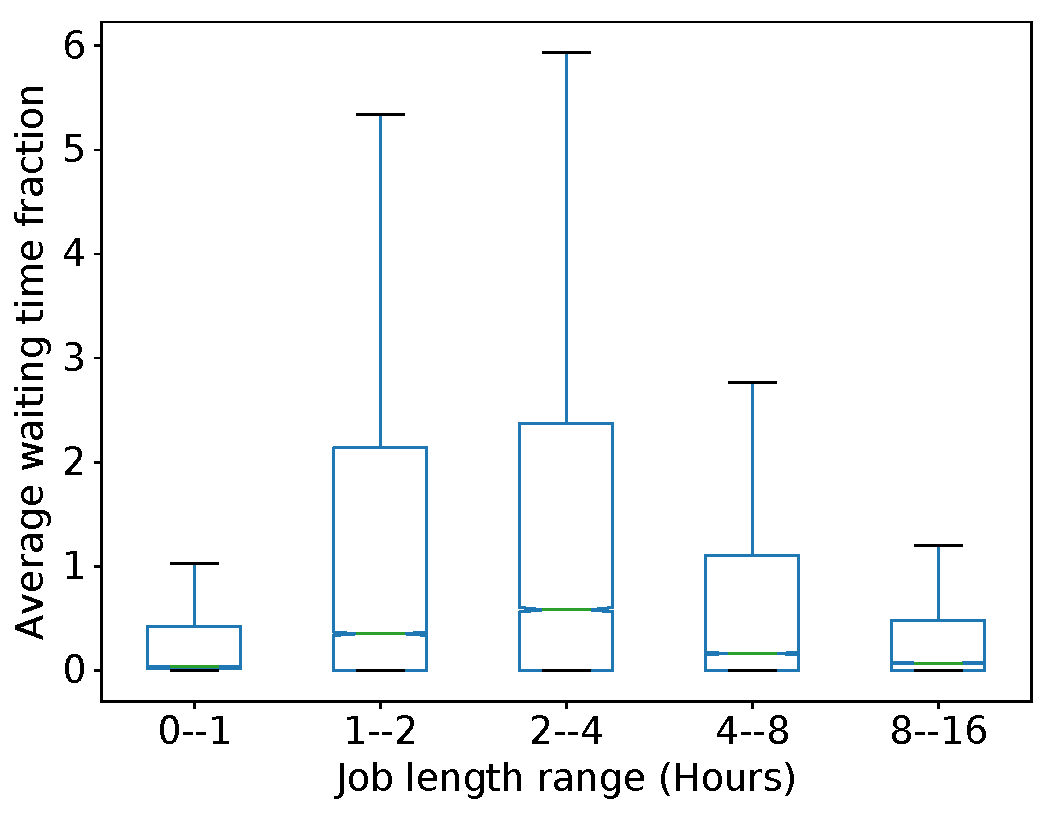
\includegraphics[width=0.4\textwidth]{../graphs/waiting_time_buckets.pdf}
  \caption{Waiting time fraction of jobs of different lengths varies.}
  \label{fig:hpc-wait-buckets}  
\end{figure}

%%% Local Variables:
%%% mode: latex
%%% TeX-master: "paper"
%%% End:
